\documentclass{anstrans}
%%%%%%%%%%%%%%%%%%%%%%%%%%%%%%%%%%%
\title{Optimal Sizing of a Micro-Reactor for Embedded Grid Systems}
\author{Samuel G. Dotson and Kathryn D. Huff}

\institute{
Dept. of Nuclear, Plasma and Radiological Engineering, University of Illinois at Urbana-Champaign \\
sgd2@illinois.edu
}

%%%% packages and definitions (optional)
\usepackage{graphicx} % allows inclusion of graphics
\graphicspath{{./../figures/}}
\usepackage{float}
\usepackage{booktabs} % nice rules (thick lines) for tables
\usepackage{microtype} % improves typography for PDF
\usepackage{xspace}
\usepackage{tabularx}
\usepackage{amsmath}
\usepackage{subcaption}
\usepackage{enumitem}
\usepackage{placeins}
\usepackage{tikz}
\usetikzlibrary{shapes.geometric, arrows}
\usepackage[acronym,toc]{glossaries}
\newacronym[longplural={metric tons of heavy metal}]{MTHM}{MTHM}{metric ton of heavy metal}
\newacronym{ABM}{ABM}{agent-based modeling}
\newacronym{ACDIS}{ACDIS}{Program in Arms Control \& Domestic and International Security}
\newacronym{AHTR}{AHTR}{Advanced High Temperature Reactor}
\newacronym{ANDRA}{ANDRA}{Agence Nationale pour la gestion des D\'echets RAdioactifs, the French National Agency for Radioactive Waste Management}
\newacronym{APP}{APP}{Abbott Power Plant}
\newacronym{ANL}{ANL}{Argonne National Laboratory}
\newacronym{API}{API}{application programming interface}
\newacronym{ARCH}{ARCH}{autoregressive conditional heteroskedastic}
\newacronym{ARE}{ARE}{Aircraft Reactor Experiment}
\newacronym{ARFC}{ARFC}{Advanced Reactors and Fuel Cycles}
\newacronym{ARMA}{ARMA}{autoregressive moving average}
\newacronym{ASME}{ASME}{American Society of Mechanical Engineers}
\newacronym{ATWS}{ATWS}{Anticipated Transient Without Scram}
\newacronym{BDBE}{BDBE}{Beyond Design Basis Event}
\newacronym{BIDS}{BIDS}{Berkeley Institute for Data Science}
\newacronym{BOL}{BOL}{Beginning-of-Life}
\newacronym{BSD}{BSD}{Berkeley Software Distribution}
\newacronym{CAFCA}{CAFCA}{ Code for Advanced Fuel Cycles Assessment }
\newacronym{CASL}{CASL}{Consortium for Advanced Simulation of Light Water Reactors}
\newacronym{CDTN}{CDTN}{Centro de Desenvolvimento da Tecnologia Nuclear}
\newacronym{CEA}{CEA}{Commissariat \`a l'\'Energie Atomique et aux \'Energies Alternatives}
\newacronym{CI}{CI}{continuous integration}
\newacronym{CNEC}{CNEC}{Consortium for Nonproliferation Enabling Capabilities}
\newacronym{CNEN}{CNEN}{Comiss\~{a}o Nacional de Energia Nuclear}
\newacronym{CNERG}{CNERG}{Computational Nuclear Engineering Research Group}
\newacronym{COSI}{COSI}{Commelini-Sicard}
\newacronym{COTS}{COTS}{commercial, off-the-shelf}
\newacronym{CSNF}{CSNF}{commercial spent nuclear fuel}
\newacronym{CTAH}{CTAHs}{Coiled Tube Air Heaters}
\newacronym{CUBIT}{CUBIT}{CUBIT Geometry and Mesh Generation Toolkit}
\newacronym{CURIE}{CURIE}{Centralized Used Fuel Resource for Information Exchange}
\newacronym{DAG}{DAG}{directed acyclic graph}
\newacronym{DANESS}{DANESS}{Dynamic Analysis of Nuclear Energy System Strategies}
\newacronym{DBE}{DBE}{Design Basis Event}
\newacronym{DESAE}{DESAE}{Dynamic Analysis of Nuclear Energy Systems Strategies}
\newacronym{DHS}{DHS}{Department of Homeland Security}
\newacronym{DOE}{DOE}{Department of Energy}
\newacronym{DRACS}{DRACS}{Direct Reactor Auxiliary Cooling System}
\newacronym{DRE}{DRE}{dynamic resource exchange}
\newacronym{DSNF}{DSNF}{DOE spent nuclear fuel}
\newacronym{DYMOND}{DYMOND}{Dynamic Model of Nuclear Development }
\newacronym{EBS}{EBS}{Engineered Barrier System}
\newacronym{EDZ}{EDZ}{Excavation Disturbed Zone}
\newacronym{EIA}{EIA}{U.S. Energy Information Administration}
\newacronym{EPA}{EPA}{Environmental Protection Agency}
\newacronym{EP}{EP}{Engineering Physics}
\newacronym{FCO}{FCO}{Fuel Cycle Options}
\newacronym{FCT}{FCT}{Fuel Cycle Technology}
\newacronym{FCWMD}{FCWMD}{Fuel Cycle and Waste Management Division}
\newacronym{FEHM}{FEHM}{Finite Element Heat and Mass Transfer}
\newacronym{FEPs}{FEPs}{Features, Events, and Processes}
\newacronym{FHR}{FHR}{Fluoride-Salt-Cooled High-Temperature Reactor}
\newacronym{FLiBe}{FLiBe}{Fluoride-Lithium-Beryllium}
\newacronym{GCAM}{GCAM}{Global Change Assessment Model}
\newacronym{GDSE}{GDSE}{Generic Disposal System Environment}
\newacronym{GDSM}{GDSM}{Generic Disposal System Model}
\newacronym{GENIUSv1}{GENIUSv1}{Global Evaluation of Nuclear Infrastructure Utilization Scenarios, Version 1}
\newacronym{GENIUSv2}{GENIUSv2}{Global Evaluation of Nuclear Infrastructure Utilization Scenarios, Version 2}
\newacronym{GENIUS}{GENIUS}{Global Evaluation of Nuclear Infrastructure Utilization Scenarios}
\newacronym{GPAM}{GPAM}{Generic Performance Assessment Model}
\newacronym{GRSAC}{GRSAC}{Graphite Reactor Severe Accident Code}
\newacronym{GUI}{GUI}{graphical user interface}
\newacronym{HLW}{HLW}{high level waste}
\newacronym{HPC}{HPC}{high-performance computing}
\newacronym{HTC}{HTC}{high-throughput computing}
\newacronym{HTGR}{HTGR}{High Temperature Gas-Cooled Reactor}
\newacronym{IAEA}{IAEA}{International Atomic Energy Agency}
\newacronym{IEMA}{IEMA}{Illinois Emergency Mangament Agency}
\newacronym{INL}{INL}{Idaho National Laboratory}
\newacronym{IPRR1}{IRP-R1}{Instituto de Pesquisas Radioativas Reator 1}
\newacronym{IRP}{IRP}{Integrated Research Project}
\newacronym{ISFSI}{ISFSI}{Independent Spent Fuel Storage Installation}
\newacronym{ISRG}{ISRG}{Independent Student Research Group}
\newacronym{JFNK}{JFNK}{Jacobian-Free Newton Krylov}
\newacronym{LANL}{LANL}{Los Alamos National Laboratory}
\newacronym{LBNL}{LBNL}{Lawrence Berkeley National Laboratory}
\newacronym{LCOE}{LCOE}{levelized cost of electricity}
\newacronym{LDRD}{LDRD}{laboratory directed research and development}
\newacronym{LFR}{LFR}{Lead-Cooled Fast Reactor}
\newacronym{LGPL}{LGPL}{Lesser GNU Public License}
\newacronym{LLNL}{LLNL}{Lawrence Livermore National Laboratory}
\newacronym{LMFBR}{LMFBR}{Liquid-Metal-cooled Fast Breeder Reactor}
\newacronym{LOFC}{LOFC}{Loss of Forced Cooling}
\newacronym{LOHS}{LOHS}{Loss of Heat Sink}
\newacronym{LOLA}{LOLA}{Loss of Large Area}
\newacronym{LP}{LP}{linear program}
\newacronym{LWR}{LWR}{Light Water Reactor}
\newacronym{MARKAL}{MARKAL}{MARKet and ALlocation}
\newacronym{MA}{MA}{minor actinide}
\newacronym{MCNP}{MCNP}{Monte Carlo N-Particle code}
\newacronym{MILP}{MILP}{mixed-integer linear program}
\newacronym{MIT}{MIT}{the Massachusetts Institute of Technology}
\newacronym{MOAB}{MOAB}{Mesh-Oriented datABase}
\newacronym{MOOSE}{MOOSE}{Multiphysics Object-Oriented Simulation Environment}
\newacronym{MOX}{MOX}{mixed oxide}
\newacronym{MSBR}{MSBR}{Molten Salt Breeder Reactor}
\newacronym{MSRE}{MSRE}{Molten Salt Reactor Experiment}
\newacronym{MSR}{MSR}{Molten Salt Reactor}
\newacronym{NAGRA}{NAGRA}{National Cooperative for the Disposal of Radioactive Waste}
\newacronym{NCSA}{NCSA}{National Center for Supercomputing Applications}
\newacronym{NEAMS}{NEAMS}{Nuclear Engineering Advanced Modeling and Simulation}
\newacronym{NEUP}{NEUP}{Nuclear Energy University Programs}
\newacronym{NFCSim}{NFCSim}{Nuclear Fuel Cycle Simulator}
\newacronym{NFC}{NFC}{Nuclear Fuel Cycle}
\newacronym{NGNP}{NGNP}{Next Generation Nuclear Plant}
\newacronym{NMWPC}{NMWPC}{Nuclear MW Per Capita}
\newacronym{NNSA}{NNSA}{National Nuclear Security Administration}
\newacronym{NPRE}{NPRE}{Department of Nuclear, Plasma, and Radiological Engineering}
\newacronym{NQA1}{NQA-1}{Nuclear Quality Assurance - 1}
\newacronym{NRC}{NRC}{Nuclear Regulatory Commission}
\newacronym{NSF}{NSF}{National Science Foundation}
\newacronym{NSSC}{NSSC}{Nuclear Science and Security Consortium}
\newacronym{NUWASTE}{NUWASTE}{Nuclear Waste Assessment System for Technical Evaluation}
\newacronym{NWF}{NWF}{Nuclear Waste Fund}
\newacronym{NWTRB}{NWTRB}{Nuclear Waste Technical Review Board}
\newacronym{OCRWM}{OCRWM}{Office of Civilian Radioactive Waste Management}
\newacronym{ORION}{ORION}{ORION}
\newacronym{ORNL}{ORNL}{Oak Ridge National Laboratory}
\newacronym{PARCS}{PARCS}{Purdue Advanced Reactor Core Simulator}
\newacronym{PBAHTR}{PB-AHTR}{Pebble Bed Advanced High Temperature Reactor}
\newacronym{PBFHR}{PB-FHR}{Pebble-Bed Fluoride-Salt-Cooled High-Temperature Reactor}
\newacronym{PEI}{PEI}{Peak Environmental Impact}
\newacronym{PH}{PRONGHORN}{PRONGHORN}
\newacronym{PI}{PI}{Principal Investigator}
\newacronym{PNNL}{PNNL}{Pacific Northwest National Laboratory}
\newacronym{PRIS}{PRIS}{Power Reactor Information System}
\newacronym{PRKE}{PRKE}{Point Reactor Kinetics Equations}
\newacronym{PSPG}{PSPG}{Pressure-Stabilizing/Petrov-Galerkin}
\newacronym{PWAR}{PWAR}{Pratt and Whitney Aircraft Reactor}
\newacronym{PWR}{PWR}{Pressurized Water Reactor}
\newacronym{PyNE}{PyNE}{Python toolkit for Nuclear Engineering}
\newacronym{PyRK}{PyRK}{Python for Reactor Kinetics}
\newacronym{QA}{QA}{quality assurance}
\newacronym{RDD}{RD\&D}{Research Development and Demonstration}
\newacronym{RD}{R\&D}{Research and Development}
\newacronym{RELAP}{RELAP}{Reactor Excursion and Leak Analysis Program}
\newacronym{RIA}{RIA}{Reactivity Insertion Accident}
\newacronym{RIF}{RIF}{Region-Institution-Facility}
\newacronym{SAM}{SAM}{Simulation and Modeling}
\newacronym{SCF}{SCF}{Software Carpentry Foundation}
\newacronym{SFR}{SFR}{Sodium-Cooled Fast Reactor}
\newacronym{SINDAG}{SINDA{\textbackslash}G}{Systems Improved Numerical Differencing Analyzer $\backslash$ Gaski}
\newacronym{SKB}{SKB}{Svensk K\"{a}rnbr\"{a}nslehantering AB}
\newacronym{SNF}{SNF}{spent nuclear fuel}
\newacronym{SNL}{SNL}{Sandia National Laboratory}
\newacronym{SNM}{SNM}{Special Nuclear Material}
\newacronym{STC}{STC}{specific temperature change}
\newacronym{SUPG}{SUPG}{Streamline-Upwind/Petrov-Galerkin}
\newacronym{SWF}{SWF}{Separations and Waste Forms}
\newacronym{SWU}{SWU}{Separative Work Unit}
\newacronym{SandO}{S\&O}{Signatures and Observables}
\newacronym{THW}{THW}{The Hacker Within}
\newacronym{TRIGA}{TRIGA}{Training Research Isotope General Atomic}
\newacronym{TRISO}{TRISO}{Tristructural Isotropic}
\newacronym{TSM}{TSM}{Total System Model}
\newacronym{TSPA}{TSPA}{Total System Performance Assessment for the Yucca Mountain License Application}
\newacronym{UDB}{UDB}{Unified Database}
\newacronym{UFD}{UFD}{Used Fuel Disposition}
\newacronym{UML}{UML}{Unified Modeling Language}
\newacronym{UNFSTANDARDS}{UNFST\&DARDS}{Used Nuclear Fuel Storage, Transportation \& Disposal Analysis Resource and Data System}
\newacronym{UOX}{UOX}{uranium oxide}
\newacronym{UQ}{UQ}{uncertainty quantification}
\newacronym{US}{US}{United States}
\newacronym{UW}{UW}{University of Wisconsin}
\newacronym{VISION}{VISION}{the Verifiable Fuel Cycle Simulation Model}
\newacronym{VV}{V\&V}{verification and validation}
\newacronym{WIPP}{WIPP}{Waste Isolation Pilot Plant}
\newacronym{YMG}{YMG}{Young Members Group}
\newacronym{YMR}{YMR}{Yucca Mountain Repository Site}
\newacronym{NEI}{NEI}{Nuclear Energy Institute}
%\newacronym{<++>}{<++>}{<++>}
%\newacronym{<++>}{<++>}{<++>}

\makeglossaries

\newcolumntype{c}{>{\hsize=.56\hsize}X}
\newcolumntype{b}{>{\hsize=.7\hsize}X}
\newcolumntype{s}{>{\hsize=.74\hsize}X}
\newcolumntype{f}{>{\hsize=.1\hsize}X}
\newcolumntype{a}{>{\hsize=.45\hsize}X}
\usepackage{titlesec}
\titleformat*{\subsection}{\normalfont}

\begin{document}

%%%%%%%%%%%%%%%%%%%%%%%%%%%%%%%%%%%%%%%%%%%%%%%%%%%%%%%%%%%%%%%%%%%%%%%%%%%%%%%%%
% define the tikz style
\tikzstyle{rect} = [draw, rectangle, fill=white!20,text width=6em, text centered, minimum height=2em]
\tikzstyle{elli} = [draw, ellipse, fill=white!20,text width=6em, text centered, minimum height=2em]
\tikzstyle{circ} = [draw, circle, fill=white!20,text width=6em, text centered, inn sep = 10pt]
\tikzstyle{diam} = [draw, diamond, fill=white!20,text width=6em, text badly centered, inner sep=0pt]
\tikzstyle{line} = [draw, -latex']

%%%%%%%%%%%%%%%%%%%%%%%%%%%%%%%%%%%%%%%%%%%%%%%%%%%%%%%%%%%%%%%%%%%%%%%%%%%%%%%%
\begin{frame}
\frametitle{Introduction}
\begin{columns}
    \column[t]{5cm}
	\begin{figure}[htbp!]
		\begin{center}
			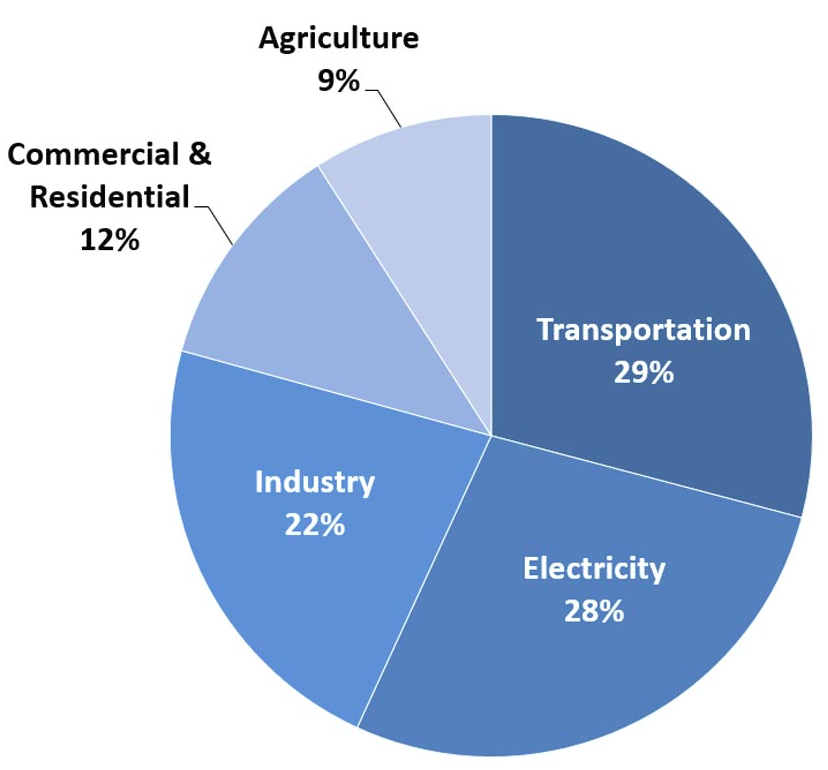
\includegraphics[height=6.2cm]{images/total-ghg-2017.png}
		\end{center}
		\caption{Total U.S. GHG Emissions by Economic Sector in 2017 \cite{us_epa_sources_2020}.}
	\end{figure}

	\column[t]{5cm}
	\begin{itemize}
		\item Illinois Climate Action Plan (iCAP).
		\item Attain carbon neutrality by 2050.
	\end{itemize}
\end{columns}
\end{frame}

% Notes:
% Transportation and Electricity are the economic sectors that produced ...

\begin{frame}
\frametitle{Transportation}
\begin{columns}
	\column[t]{5cm}
	\begin{itemize}
		\item Hydrogen economy
		\item california, japan, germany
	\end{itemize}

% Maybe a figure?
 %    \column[t]{5cm}
	% \begin{figure}[htbp!]
	% 	\begin{center}
	% 		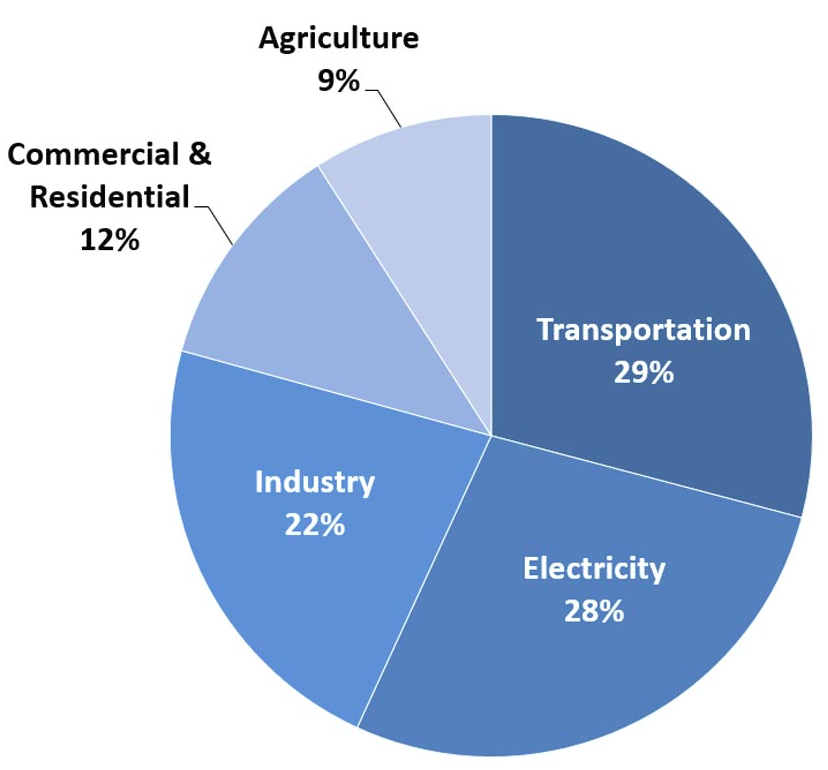
\includegraphics[height=6.2cm]{images/total-ghg-2017.png}
	% 	\end{center}
	% 	\caption{Total U.S. GHG Emissions by Economic Sector in 2017 \cite{us_epa_sources_2020}.}
	% \end{figure}
\end{columns}
\end{frame}

\begin{frame}
\frametitle{Electricity}
\begin{columns}
	\column[t]{5cm}
	\begin{itemize}
		\item More renewables
		\item Duck curve
	\end{itemize}

% Maybe a figure?
 %    \column[t]{5cm}
	% \begin{figure}[htbp!]
	% 	\begin{center}
	% 		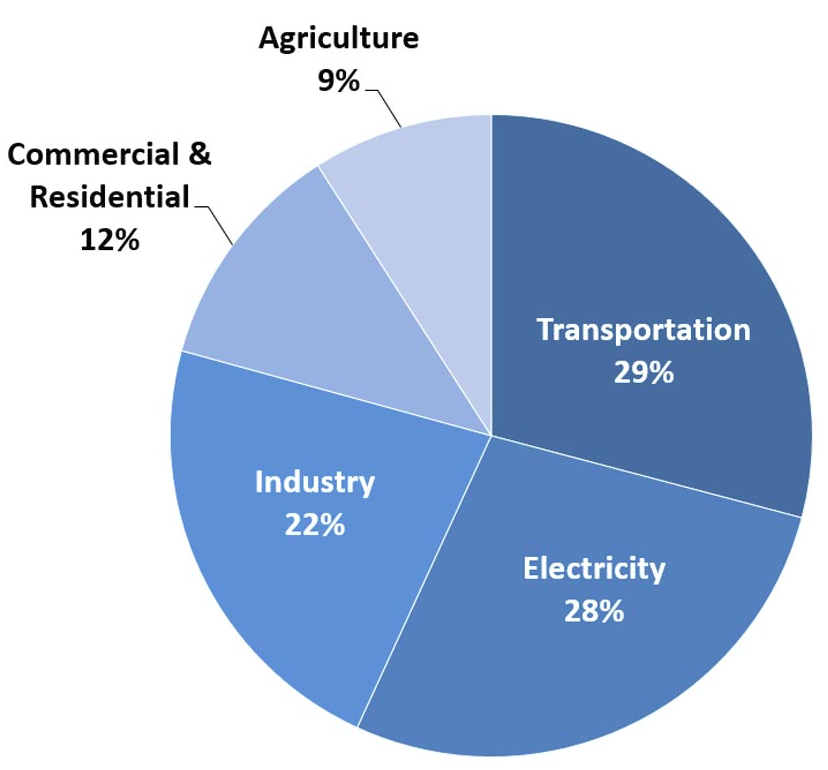
\includegraphics[height=6.2cm]{images/total-ghg-2017.png}
	% 	\end{center}
	% 	\caption{Total U.S. GHG Emissions by Economic Sector in 2017 \cite{us_epa_sources_2020}.}
	% \end{figure}
\end{columns}
\end{frame}

















% \begin{frame}
% \frametitle{"There must be something wrong at SL-1"}
% \begin{columns}
%     \column[t]{5cm}
% 	\begin{itemize}
% 		\item 9:01 pm alarm goes off at the main firehouse.
% 		\item Radiation readings too high, no signs of the crew.
% 		\item Ed Vallario went inside and saw Jack Byrnes.
% 		\item Retrieval of Byrnes and finding  of Legg.
% 		\item Byrnes was pronounced dead at 11:14 PM.
% 		\item Another group found the 3rd member pinned to the roof.
% 	\end{itemize}

%     \column[t]{5cm}
% 	\begin{itemize}
%         \item Retrieval of Legg's body.
%         \item Retrieval of McKinley's body.
%         \item Bodies taken to processing plant.
% 	\end{itemize}

%     "We got a reading on the detector, that by todays' standards, you'd have gotten the hell out of there." \textit{Lamprecht}.
%     \\
%     "I went to take a breath and it was like there was no more oxygen in the tank." \textit{Vallario}.

% \end{columns}
% \end{frame}

% \begin{frame}
% \frametitle{The accident}
% \begin{columns}
%     \column[t]{5cm}
% 	\begin{figure}[htbp!]
% 		\begin{center}
% 			\includegraphics[height=4.5cm]{./images/crew1a.png}
% 		\end{center}
% 		\caption{Reactor crew positions before the accident \cite{mckeown2003idaho}.}
% 	\end{figure}

%     \column[t]{5cm}
% 	\begin{itemize}
% 		\item Central rod is withdrawn 20".
% 		\item Reactor goes critical at 16.7".
% 		\item Fuel plates vaporize, water gets to 3740$^{\circ}$ F.
% 		\item Center fuel elements and central control blade ejected.
% 		\item Vessel rises out of its sheat and hits the ceiling.
% 		\item Vessel falls down.
% 	\end{itemize}
% \end{columns}
% \end{frame}


% \begin{frame}
% \frametitle{Theories}

% ”The direct cause of the incident clearly appears to have been the manual withdrawal by one or more of the maintenance crew of the central control rod blade from the SL-1 core considerably beyond the limit specified in the maintenance procedure. The reason or motive for the abnormal withdrawal is considered highly speculative, and it does not appear at all likely that there will ever be any reasons to change this judgment.”

% \end{frame}

% \begin{frame}
% \frametitle{Evaluation}
% 	\begin{block}{Author and Audience}
% 		\begin{itemize}
% 			\item Sources: Interviews and official documents.
% 			\item Wide audience.
% 		\end{itemize}
% 	\end{block}

% 	\begin{block}{Technical Evaluation}
% 		\begin{itemize}
% 			\item Technical explanation is not too extensive.
% 			\item A lot of details on the post-accident procedures.
% 			\item Description of the autopsies is extremely detailed.
% 		\end{itemize}
% 	\end{block}

% 	\begin{block}{Non-Technical Evaluation}
% 		\begin{itemize}
% 			\item Anecdotes, feelings, and opinions.
% 			\item Several theories on why Byrnes pulled from the rod.
% 			\item Verifiability is lost.
% 		\end{itemize}
% 	\end{block}
% \end{frame}

%%%%%%%%%%%%%%%%%%%%%%%%%%%%%%%%%%%%%%%%%%%%%%%%%%%%%%%%%%%%%%%%%%%%%%%%%%%%%%%%
\input{motivation}
 
%%%%%%%%%%%%%%%%%%%%%%%%%%%%%%%%%%%%%%%%%%%%%%%%%%%%%%%%%%%%%%%%%%%%%%%%%%%%%%%%
\section{Background}
The University of Illinois at Urbana-Champaign is an ideal model system for
this work because of its diverse energy mix. Previous work has been done to
characterize this energy grid and optimize the size of a nuclear reactor \cite{dotson_optimal_2020}. Due to the degree of wind penetration, the University is sometimes
forced to sell electricity back to MISO at a loss because of overproduction
from wind energy. Thus, a reliable prediction of electricity production from
wind and other variable sources will reduce the likelihood of these events,
specifically. In general, this prediction will also allow nuclear power plants
to bid on the wholesale market, rather than act as price takers.
\acrshort{ESN}s, a flavor of reservoir computing, are a modern
machine learning algorithm that enables accurate short
to medium term predictions. Pathak et. al used an \acrshort{ESN} to predict the
evolution of a chaotic system, a laminar flame front, up to seven Lyapunov
times in the future \cite{pathak_model-free_2018, wikner_combining_2020}. A
Lyapunov time simply measures the timescale at which chaos makes initial
predictions useless. The effect of chaos typically overwhelms conventional
predictions after a single Lyapunov time, by definition.
The Lyapunov time for a weather system is on the order of a few days but
depends on regional environment. \acrshort{ESN}s have also been used to
forecast multivariate time series
\cite{bianchi_reservoir_2020}. Echo state networks are unique among neural
networks in their ease of implementation and training speed. This is owed to its
sparse network architecture \cite{pathak_model-free_2018,
wikner_combining_2020, vannitsem_predictability_2017}. However,
their simplicity is balanced by the need for carefully chosen hyperparameters
for the desired task \cite{lukosevicius_practical_2012}.
Combining accurate demand predictions with reliable
renewable energy predictions will enable an artificially intelligent reactor
operator to adjust power in a relaxed manner.

 
%%%%%%%%%%%%%%%%%%%%%%%%%%%%%%%%%%%%%%%%%%%%%%%%%%%%%%%%%%%%%%%%%%%%%%%%%%%%%%%%
\section{Methodology}

In this work we use and extend the methodology described in Baker et. al using the \texttt{RAVEN} framework \cite{baker_optimal_2018,alfonsi_raven_2016}. This methodology allows for empirical quantification of energy system flexibility. Baker et. al used a fixed amount of nuclear power production from a small modular reactor (300 MWe) and varied the penetration of VRE in the form of wind power. They also included grid flexibility in the form of a fixed amount of battery storage. UIUC has wind and solar power purchase agreements that fix the amount of VRE the campus receives. Rather than fixing the nuclear power production, this methodology will be extended to search for the optimal size of a micro-reactor for the campus. \\
There are three main steps to this methodology \cite{baker_optimal_2018}: 

\begin{enumerate}
	\item Generate synthetic data by training a reduced order model (ROM) with historical data using \texttt{RAVEN}'s \texttt{TrainARMA} functionality. \texttt{RAVEN} condenses historical data into a typical time series and attempts to remove anomalous data.
	\item Calculate the net demand for each history set.
	\item Pass the net demand to the nuclear hybrid energy system (NHES) dispatch model defined for the UIUC embedded grid. 
\end{enumerate}

\subsection{Net Demand}
Similar to Baker et. al, we define the net demand to be 


\begin{equation}
	\label{eqn:net-demand}
	\begin{split}
		D_{net} & = (D_{total} - P_{wind} - P_{pv})_h \text{ $\forall$ $h$ in } [0,8759]
	\end{split}
\end{equation}

Where $D_{total}$ is the total demand at a given hour, $h$, of a synthetic demand profile from the ARMA model. We adjust the net demand, $D_{net}$, because VRE is used regardless of demand (thus it could exceed demand). $P_{wind}$ is computed by \cite{garcia_nuclear_2015}:

\begin{align}
	P_{wind} &= \begin{cases}
		0 &\text{ if $U_h \geq 25$}\\
		0.5\eta\rho U_h^3\frac{\pi d^2}{4} &\text{ $3 < U_h \leq 12$}\\
		8.6 &\text{ $12 < U_h < 25$}\\
	\end{cases}
\end{align}

\begin{align*}
	\intertext{where}
	\eta &\text{ is the conversion efficiency (0.31)}\\
	\rho &\text{ is the density of air at the site}\\
	U &\text{ is the wind speed in [m/s]}\\
	d &\text{ is the diameter of the turbine blades (77 m)}
\end{align*}

The value for peak output is based on the UIUC wind power purchase agreement \cite{breitweiser_wind_2016}. $P_{pv}$ is available as historical data from AlsoEnergy \cite{alsoenergy_university_2019}. There are times when the meters failed to record data so power output for those times was calculated by \cite{garcia_nuclear_2015}:

\begin{align}
 	P_{pv} &= G_T\tau_{pv}\eta_{ref}A[1-\gamma(T-25)]\\
\intertext{where}
	G_T &= DNI*\cos(\beta+\delta-lat)+DHI*\frac{180-\beta}{180}\\
	\delta &= 23.44*\sin\left(\frac{\pi}{180}\frac{360}{365}(N+284)\right)
	\intertext{where } 
	N &=\mbox{ day of the year}\nonumber\\
	DNI &=\mbox{ Direct Normal Irradiance [kW]}\nonumber\\
	DHI &=\mbox{ Diffuse Horizontal Irradiance [kW]}\nonumber\\
	G_T &=\mbox{ total irradiance [kW]}\nonumber\\
	\eta &=\mbox{ conversion efficiency (0.15)}\nonumber\\
	\beta &=\mbox{ tilt of the solar panels [$degrees$]}\nonumber\\
	\delta &=\mbox{ declination of the Earth [$degrees$]}\nonumber\\
	T &=\mbox{ temperature [$^\circ$C]}\nonumber\\
	A &=\mbox{ area covered by solar farm [$m^2$]} \nonumber\\
	\gamma &=\mbox{ temperature coefficient (0.0045)}\nonumber\\
	\tau &=\mbox{ transmittance of the PV module}\nonumber
\end{align}
These values were obtained from the iSEE facts sheet about the UIUC solar farm \cite{white_solar_2017}. 

\subsection{Dispatch Model}

The dispatch model is similar to that used by Baker et. al \cite{baker_optimal_2018}. The net demand is defined by 
Eq. \ref{eqn:net-demand}. The dispatch model first checks if renewables satisfy the campus grid demand. This can never happen with the current installed renewable capacity at UIUC. Then a hypothetical micro-reactor will produce electricity to the grid. Two assumptions will be made: First, the micro-reactor will only produce electricity and not co-generate like APP; second, the micro-reactor will operate at 100\% capacity all of the time. This second assumption is a real possibility given the range of sizes we are investigating. If the reactor can meet and exceed the net demand then the dispatch model will attempt to store the surplus in the campus chilled water system. If the chilled water tank is full, then the surplus must be sold back to the grid operator (MISO) and a penalty will be incurred. When the reactor cannot meet the electric demand, APP will produce electricity to fill the difference. UIUC will rely on APP for load following because natural gas boilers can, currently, ramp more quickly than nuclear reactors. If either the demand is not covered or all surplus power is not used then a penalty is incurred.
\begin{figure}[H]
	\centering
	\label{fig:dispatch-model}
	\resizebox{\columnwidth}{!}{%begin resizebox
		\begin{tikzpicture}[node distance = 3cm, auto]
			\node [elli] (start) {Net Demand};
			\node [diam, below of=start] (check1) {Net Demand > 0?};
			\node [rect, rounded corners, right of=check1, xshift=0.5cm] (action1) {Reactor produces electricity\\to the grid};
			\node [diam, below of=action1] (check2) {Net demand met?};
			\node [diam, left of=check2, xshift=-2cm] (check3) {Thermal storage full?};
			\node [rect, rounded corners, below of=check3] (action2) {Use surplus power to fill thermal storage};
			\node [rect, rounded corners, below of=check2, xshift=2cm] (action3) {Abbott Power Plant produces electricity to grid};
			\node [rect, rounded corners, right of=action2] (sell) {Sell surplus back to MISO};
			\node [diam, below of=action3] (check4) {Remaining demand covered?};
			\node [diam, below of=action2] (check5) {All surplus power used?};
			\node [rect, below of=check4] (penalty) {Pay Penalty};
			\node [diam, right of=check4, xshift=1cm] (hourcheck1) {hour > 8760?};
			\node [diam, left of=check5, xshift=-1cm] (hourcheck2) {hour > 8760?};

			\path[line, line width=0.5mm] (start) -- (check1);
			\path[line, line width=0.5mm] (check1) -- (action1) node [midway] {yes};
			\path[line, line width=0.5mm] (action1) -- (check2);
			\path[line, line width=0.5mm] (check2) -- (check3) node [midway] {yes};
			\path[line, line width=0.5mm] (check2) -- (action3) node [midway] {no};
			\path[line, line width=0.5mm] (check3) -- (sell) node [midway] {yes};
			\path[line, line width=0.5mm] (check3) -- (action2) node [midway] {no};
			\path[line, line width=0.5mm] (action2) -- (check5);
			\path[line, line width=0.5mm] (hourcheck2) |- (start) node [near end] {no};
 			\path[line, line width=0.5mm] (check5) -- (hourcheck2) node [midway] {yes};
			\path[line, line width=0.5mm] (check5) |- (penalty) node [near start] {no};
			\path[line, line width=0.5mm] (check4) -- (penalty) node [midway] {no};
			\path[line, line width=0.5mm] (penalty) -| (hourcheck1);
			\path[line, line width=0.5mm] (hourcheck1) |- (start) node [near end] {no};
			\path[line, line width=0.5mm] (action3) -- (check4);
			\path[line, line width=0.5mm] (check4) -- (hourcheck1) node [midway] {yes};
			\path[line, line width=0.5mm] (sell) |- (penalty);
			\path[line, line width=0.5mm] (check1) -- (check3) node [midway] {no};
		\end{tikzpicture}
	}% end resizebox
	\caption{Dispatch flow diagram for the UIUC NHES}
\end{figure}

\subsection{Capital Cost}
As in Baker et. al, capital costs are taken in full at year zero. In the first scenario we examine the simplifying assumption is that there are no capital costs because the reactor would be provided at no cost to the university. For the second scenario we will apply the model from Baker et. al. The reference plant used in that work is an 1100 MWe pressurized water reactor (PWR) which costs $\$4100$/kWh for an ideal case. $x = 0.64$ to model the economies of scale \cite{baker_optimal_2018}.

\begin{align}
	CF^{capital} &= \alpha^{year}\left(\frac{P_{\mu}}{P_{ref}}\right)^x \\
	\intertext{where}
		\alpha^{year} &= \mbox{ construction cost at year $0$}\nonumber\\
		P_\mu &= \mbox{ size of the micro-reactor}\nonumber\\
		P_{ref} &= \mbox{ size of the reference plant}\nonumber
\end{align}

%%%%%%%%%%%%%%%%%%%%%%%%%%%%%%%%%%%%%%%%%%%%%%%%%%%%%%%%%%%%%%%%%%%%%%%%%%%%%%%%
\begin{frame}
\frametitle{Transportation: fuel demand}
\begin{columns}
    \column[t]{5cm}
	\begin{figure}[htbp!]
		\begin{center}
			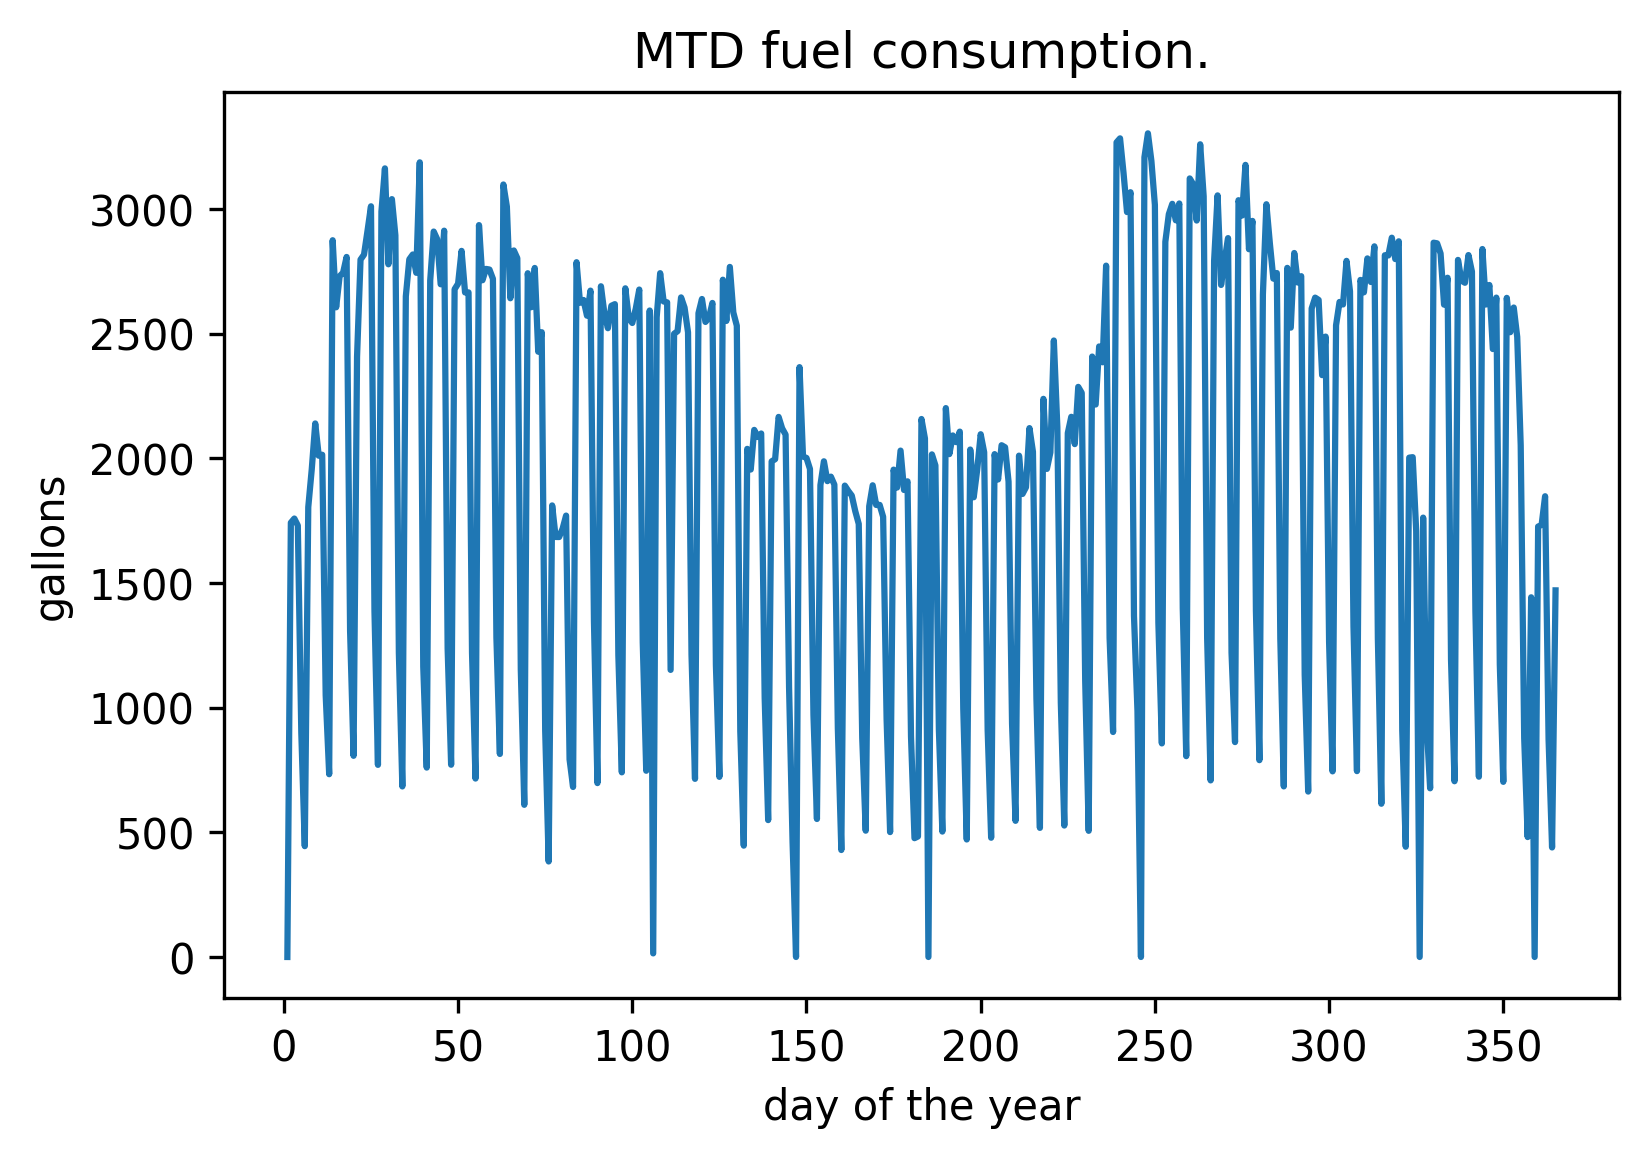
\includegraphics[height=3.5cm]{images/mtd2}
		\end{center}
		\caption{MTD fuel consumption.}
	\end{figure}

	\column[t]{5cm}
	\begin{figure}[htbp!]
		\begin{center}
			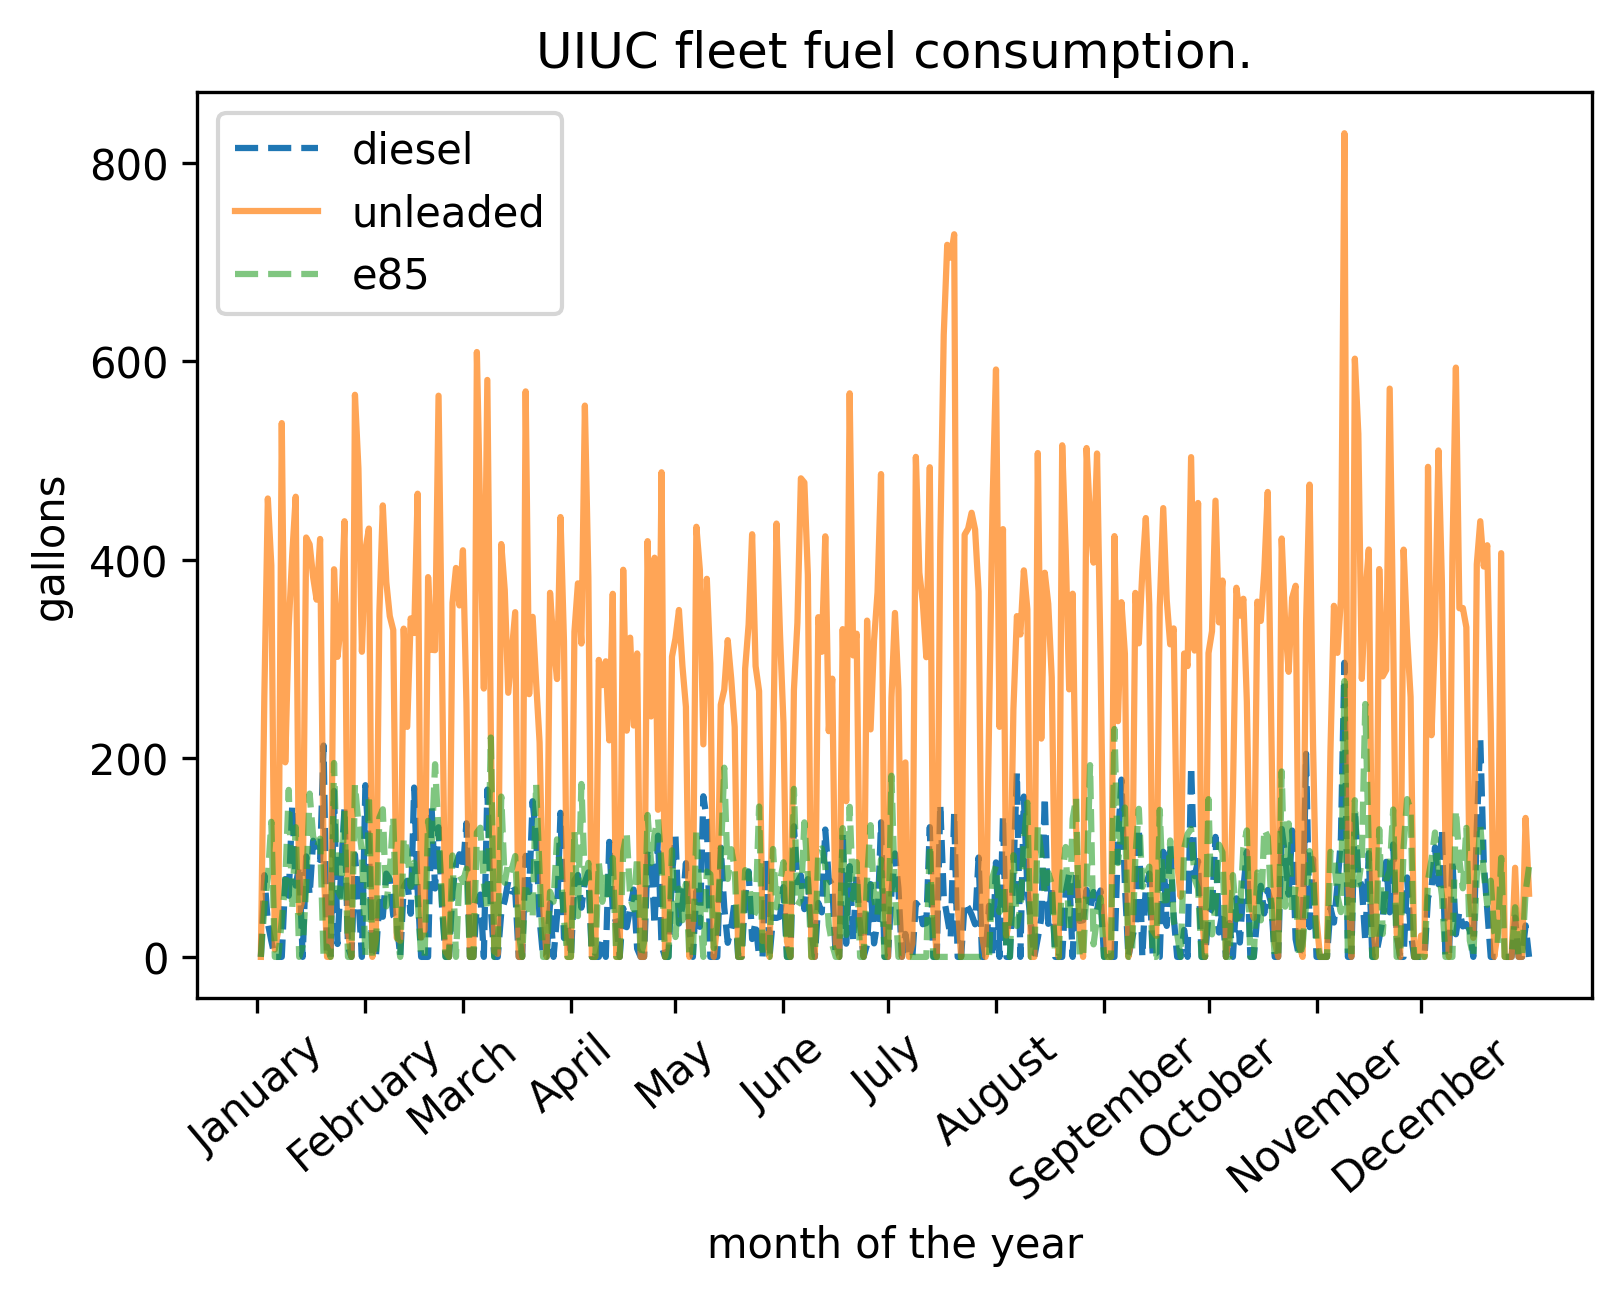
\includegraphics[height=3.5cm]{images/uiuc}
		\end{center}
		\caption{UIUC fleet fuel consumption.}
	\end{figure}
\end{columns}
\end{frame}


\begin{frame}
\frametitle{Transportation: fuel demand}
\begin{columns}
    \column[t]{5cm}
	\begin{table}[!htb]
		\centering
	    \caption{GGE, DGE, and E85GE.}
		\begin{tabular}{l|l}
		\hline
		                 & Hydrogen \\ \hline
		GGE              & 1 kg     \\
		DGE              & 1.13 kg  \\
		E85GE            & 0.78 kg  \\ \hline
        \end{tabular}
	\end{table}

	\begin{table}[!htb]
		\centering
	    \caption{Hydrogen requirements.}
		\begin{tabular}{l|l}
		\hline
		Total [kg/year]      & 943 tonnes \\
		Average [kg/day] 	 & 2584 kg    \\
		Average [kg/h] 		 & 108 kg     \\
		Maximum in one day   & 4440 kg    \\ \hline
        \end{tabular}
	\end{table}

	\column[t]{5cm}
	\begin{figure}[htbp!]
		\begin{center}
			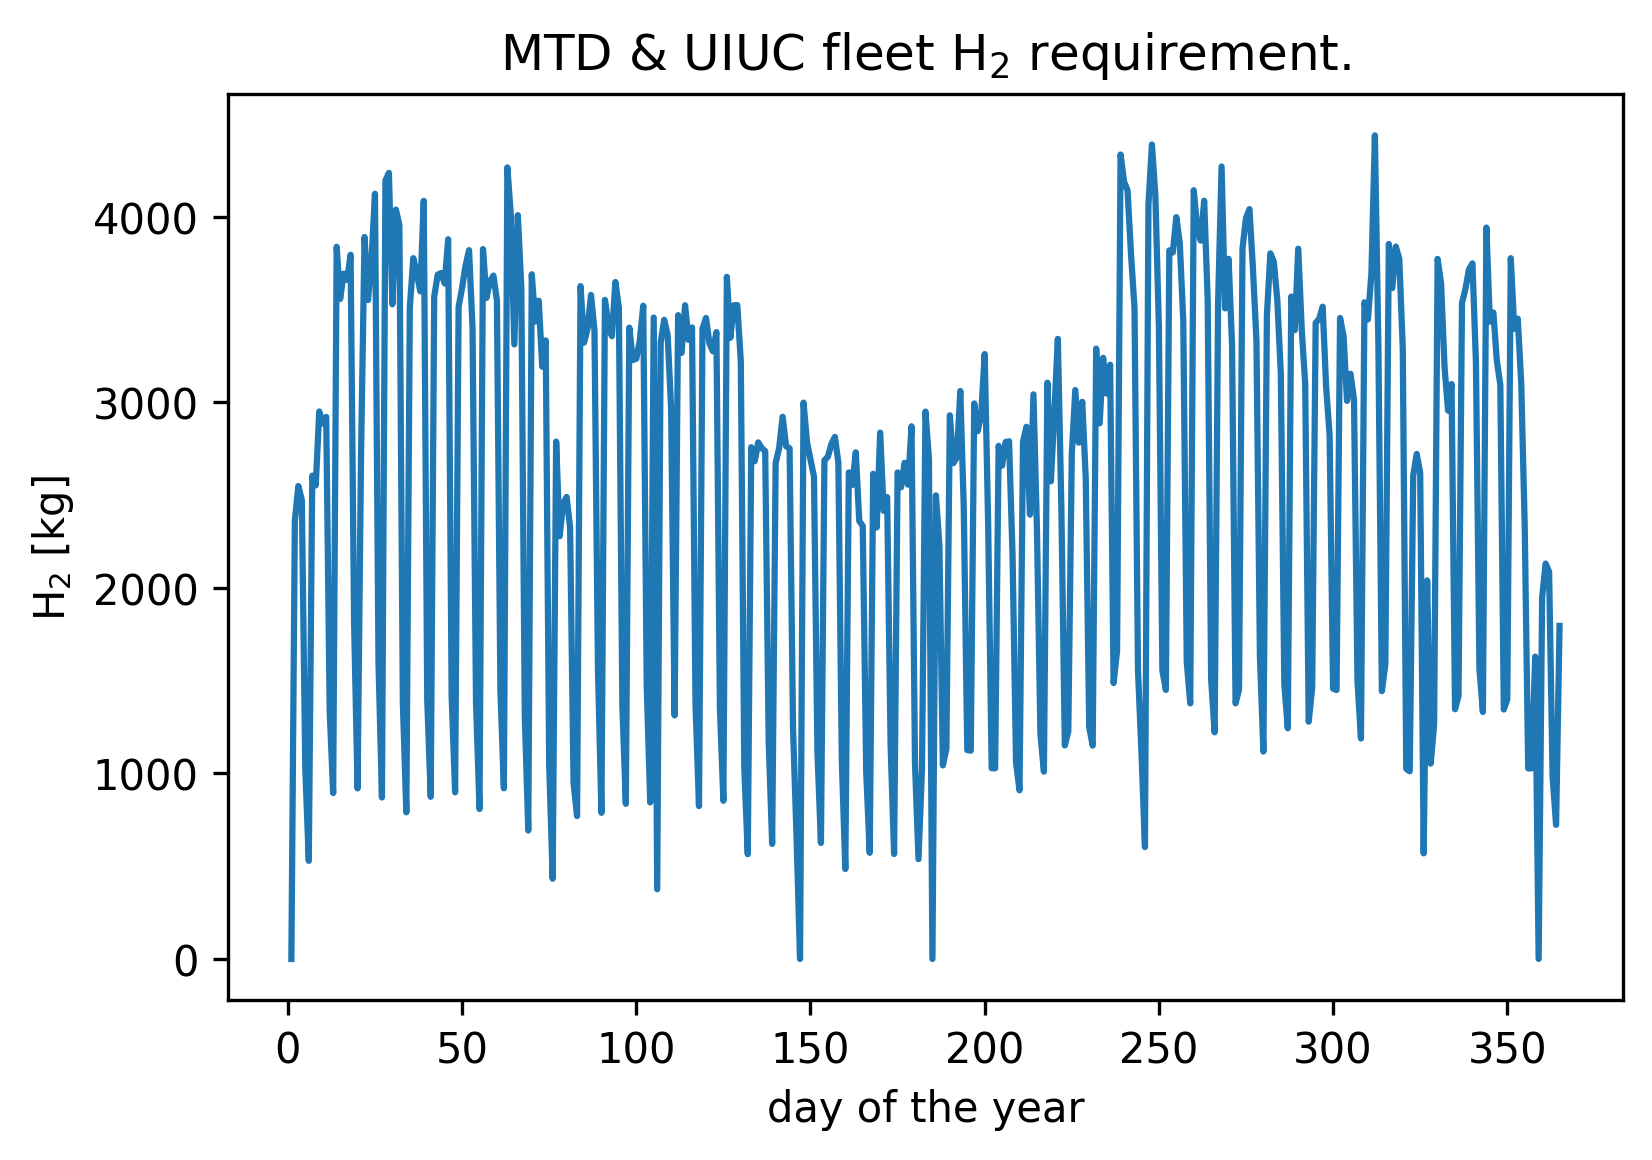
\includegraphics[height=3.5cm]{images/hydro-fleet}
		\end{center}
		\caption{MTD and UIUC fleets hydrogen requirement.}
	\end{figure}

\end{columns}
\end{frame}


\begin{frame}
\frametitle{Transportation: fuel demand}
\begin{columns}
    \column[t]{4.5cm}
	\begin{table}[!htb]
		\centering
	    \caption{Microreactor designs.}
		\begin{tabular}{l|ll}
		\hline
		Reactor      & P[MW$_{th}$] & T$_o$[$^\circ$C]\\ \hline
		MMR          & 15         & 640             \\
		eVinci       & 5          & 650             \\
		ST-OTTO      & 30         & 750             \\
		U-battery    & 10         & 750             \\
		Starcore     & 36         & 850             \\ \hline
        \end{tabular}
	\end{table}

	\column[t]{5.5cm}
	\begin{figure}[htbp!]
		\begin{center}
			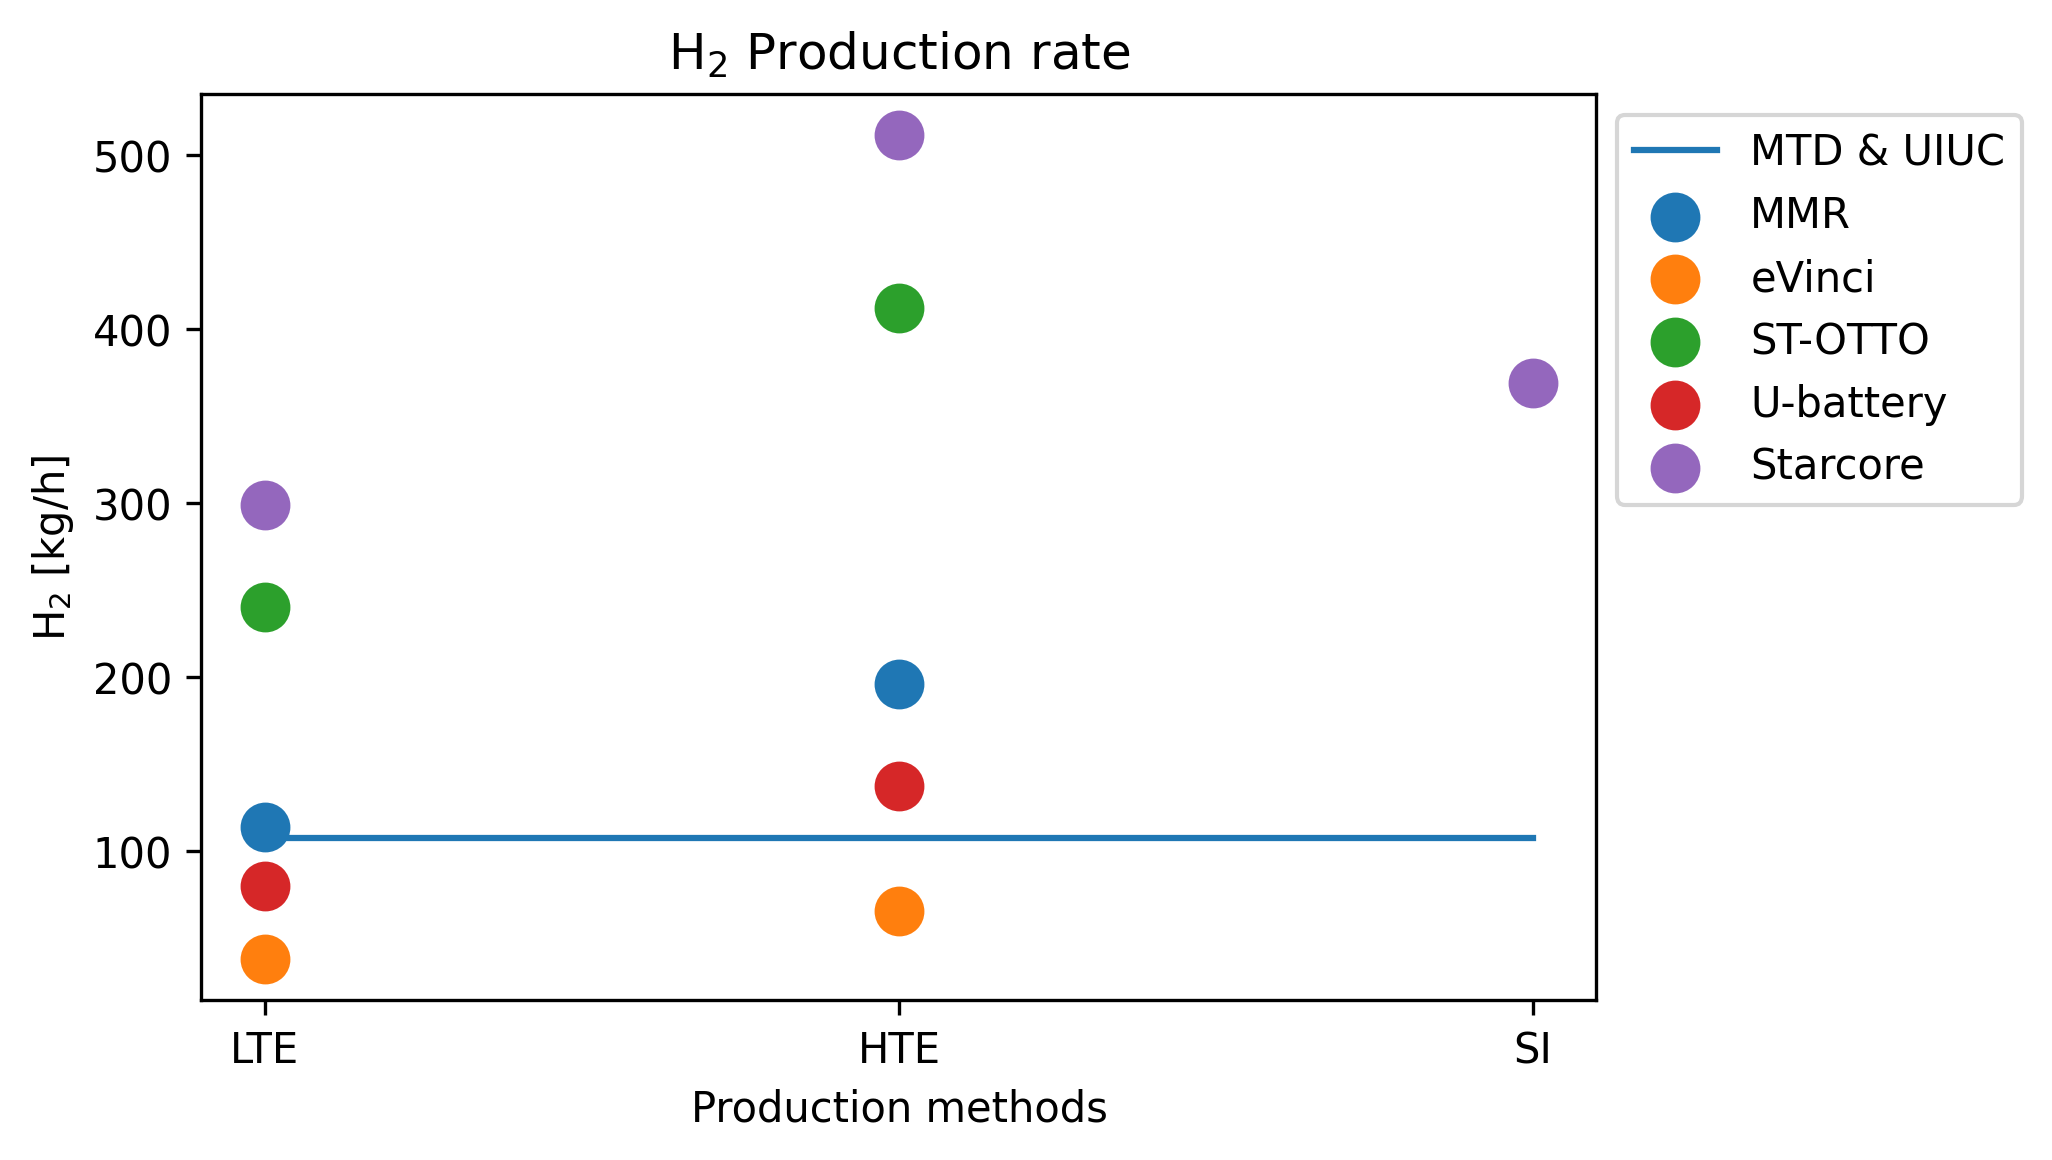
\includegraphics[height=3.5cm]{images/reactors-by-hour1}
		\end{center}
		\caption{Hydrogen production rate by different microreactor designs.}
	\end{figure}

\end{columns}
\end{frame}


\begin{frame}
\frametitle{Energy generation}
\begin{columns}
    \column[t]{5cm}
	\begin{figure}[htbp!]
		\begin{center}
			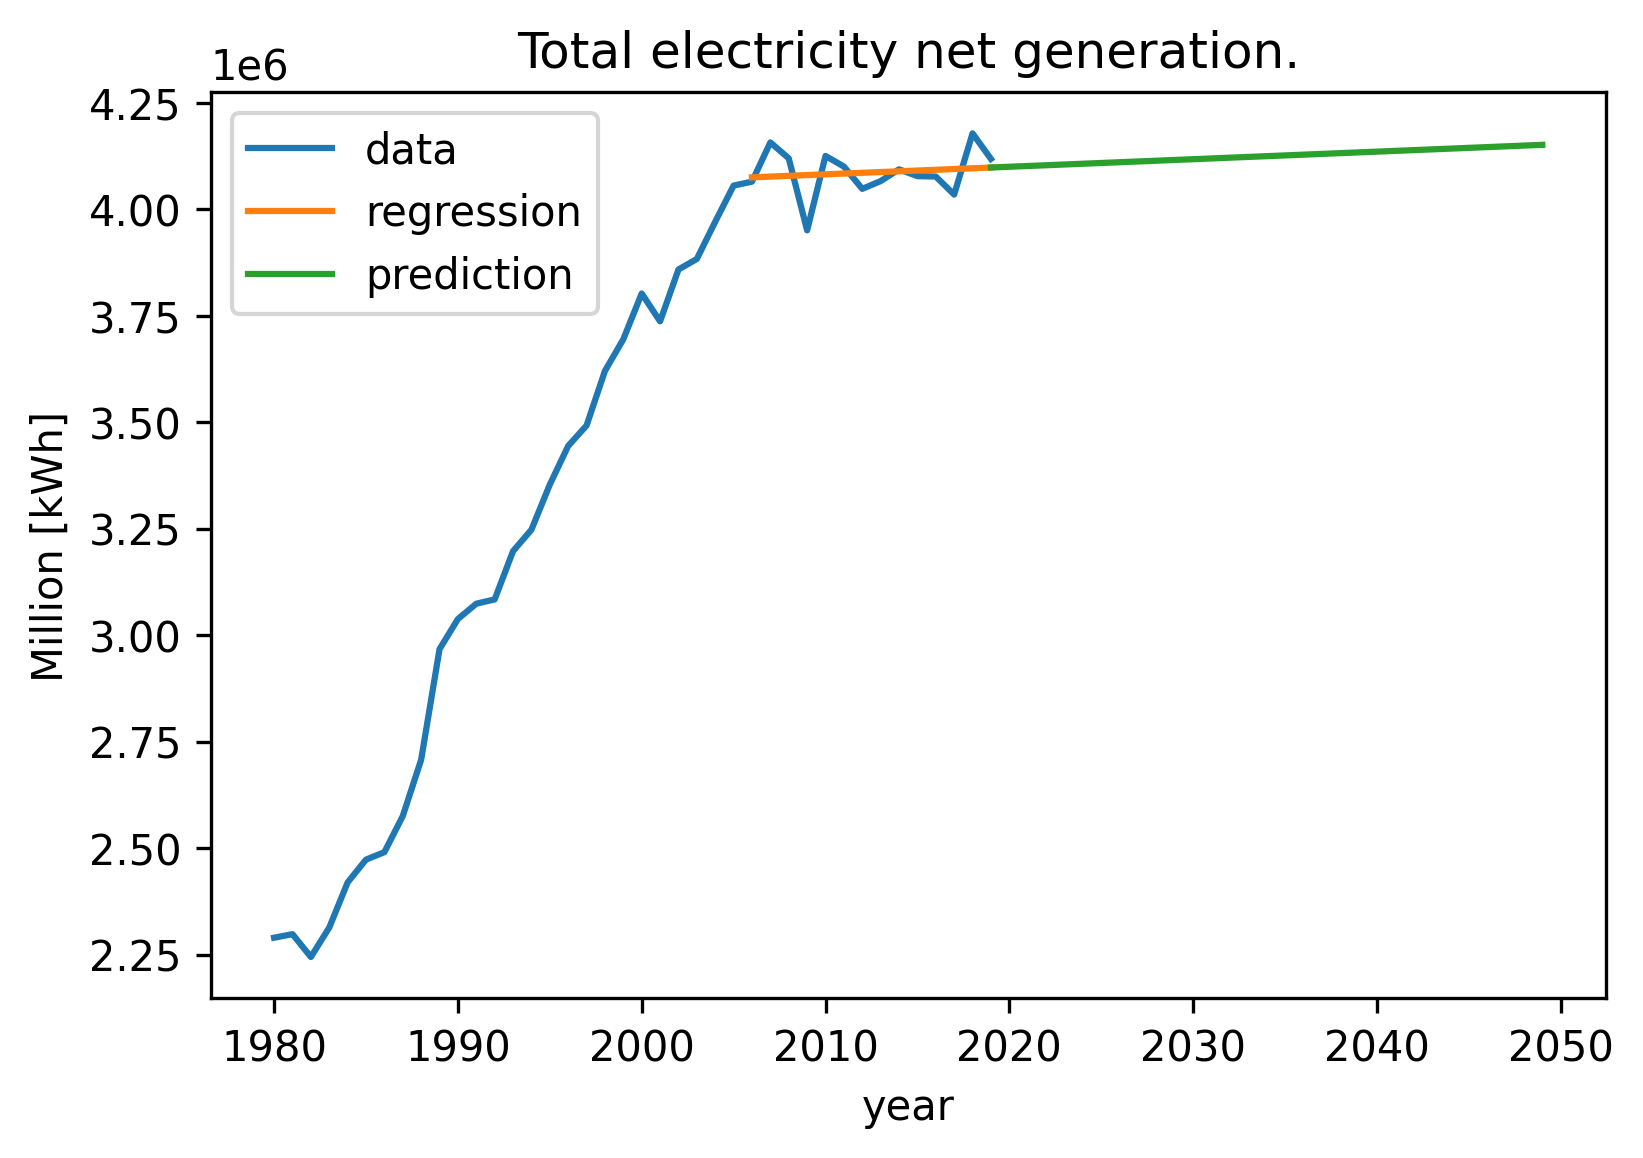
\includegraphics[height=3.3cm]{images/us-prediction1}
		\end{center}
		\caption{Prediction on the total electricity generation in the US for 2050.}
	\end{figure}

    \column[t]{5cm}
	\begin{figure}[htbp!]
		\begin{center}
			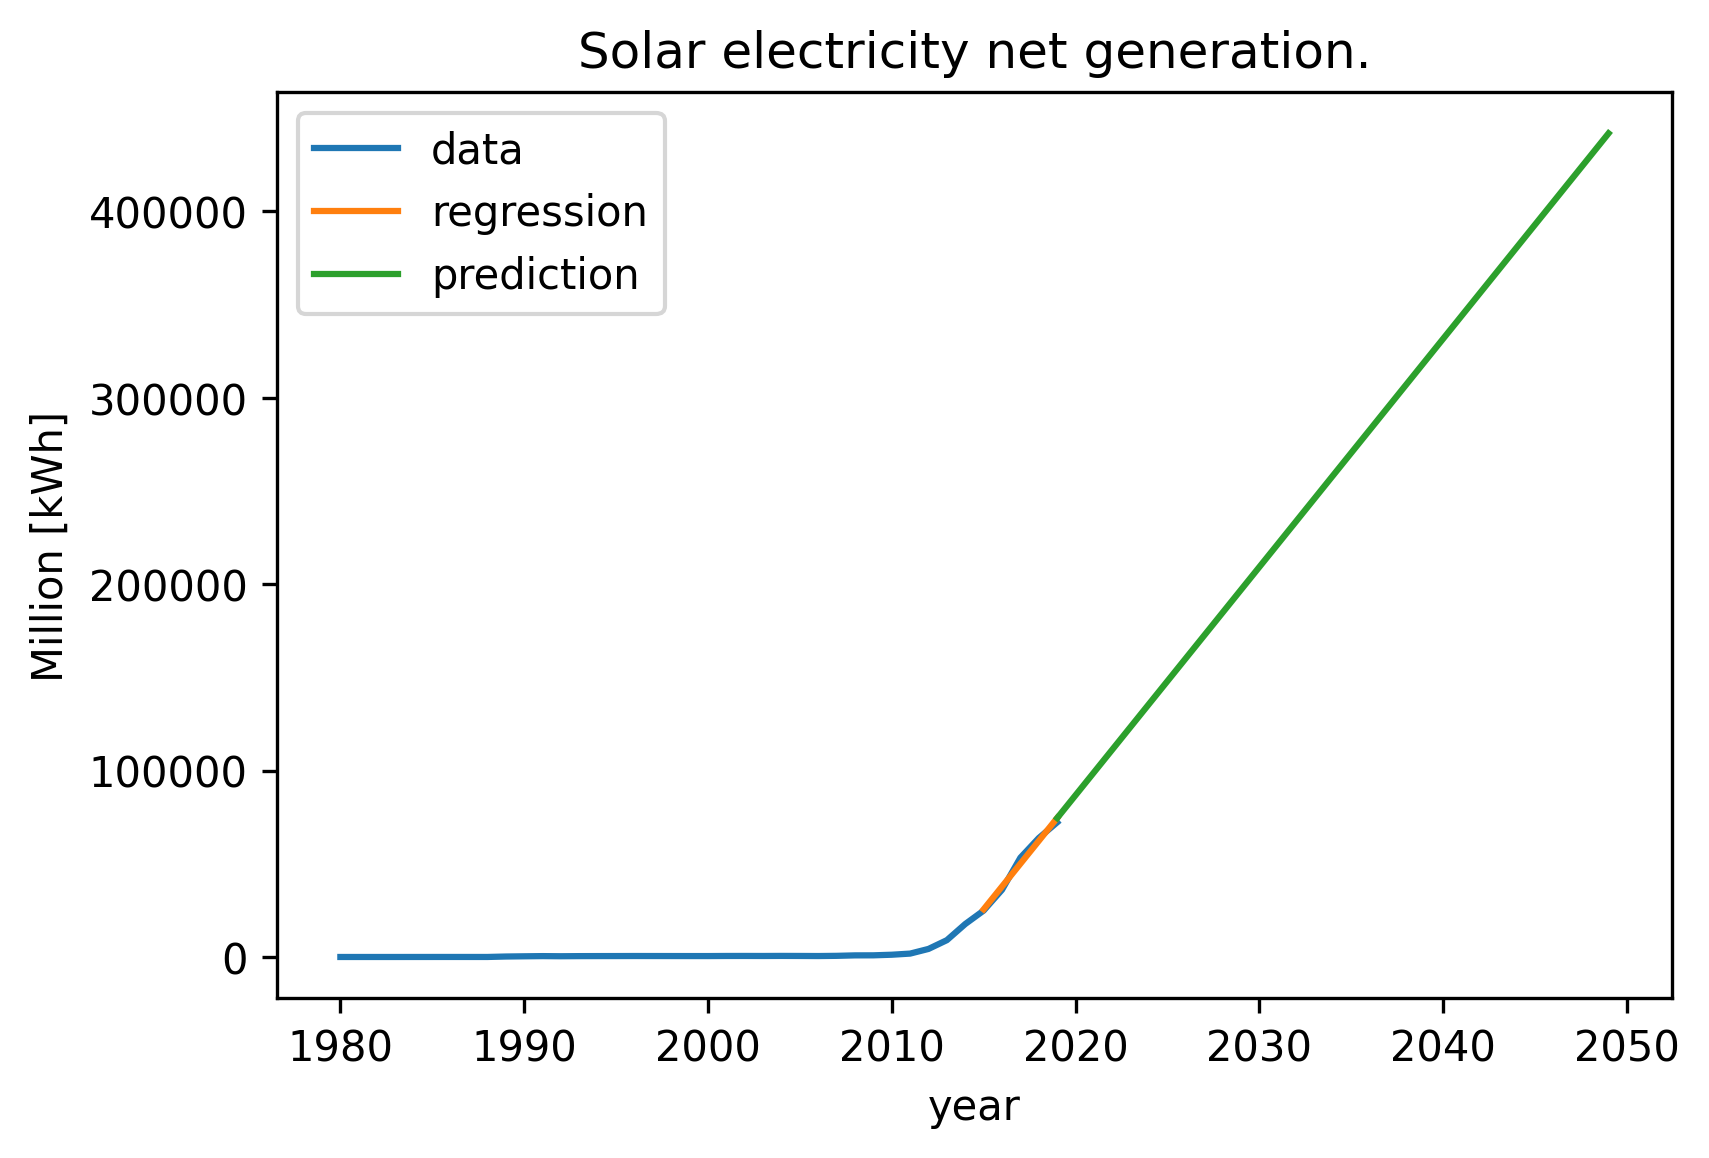
\includegraphics[height=3.3cm]{images/us-prediction2}
		\end{center}
		\caption{Prediction on the solar electricity generation in the US for 2050.}
	\end{figure}
\end{columns}
\end{frame}


\begin{frame}
\frametitle{Duck curve}
\begin{columns}
    \column[t]{4.5cm}
	\begin{figure}[htbp!]
		\begin{center}
			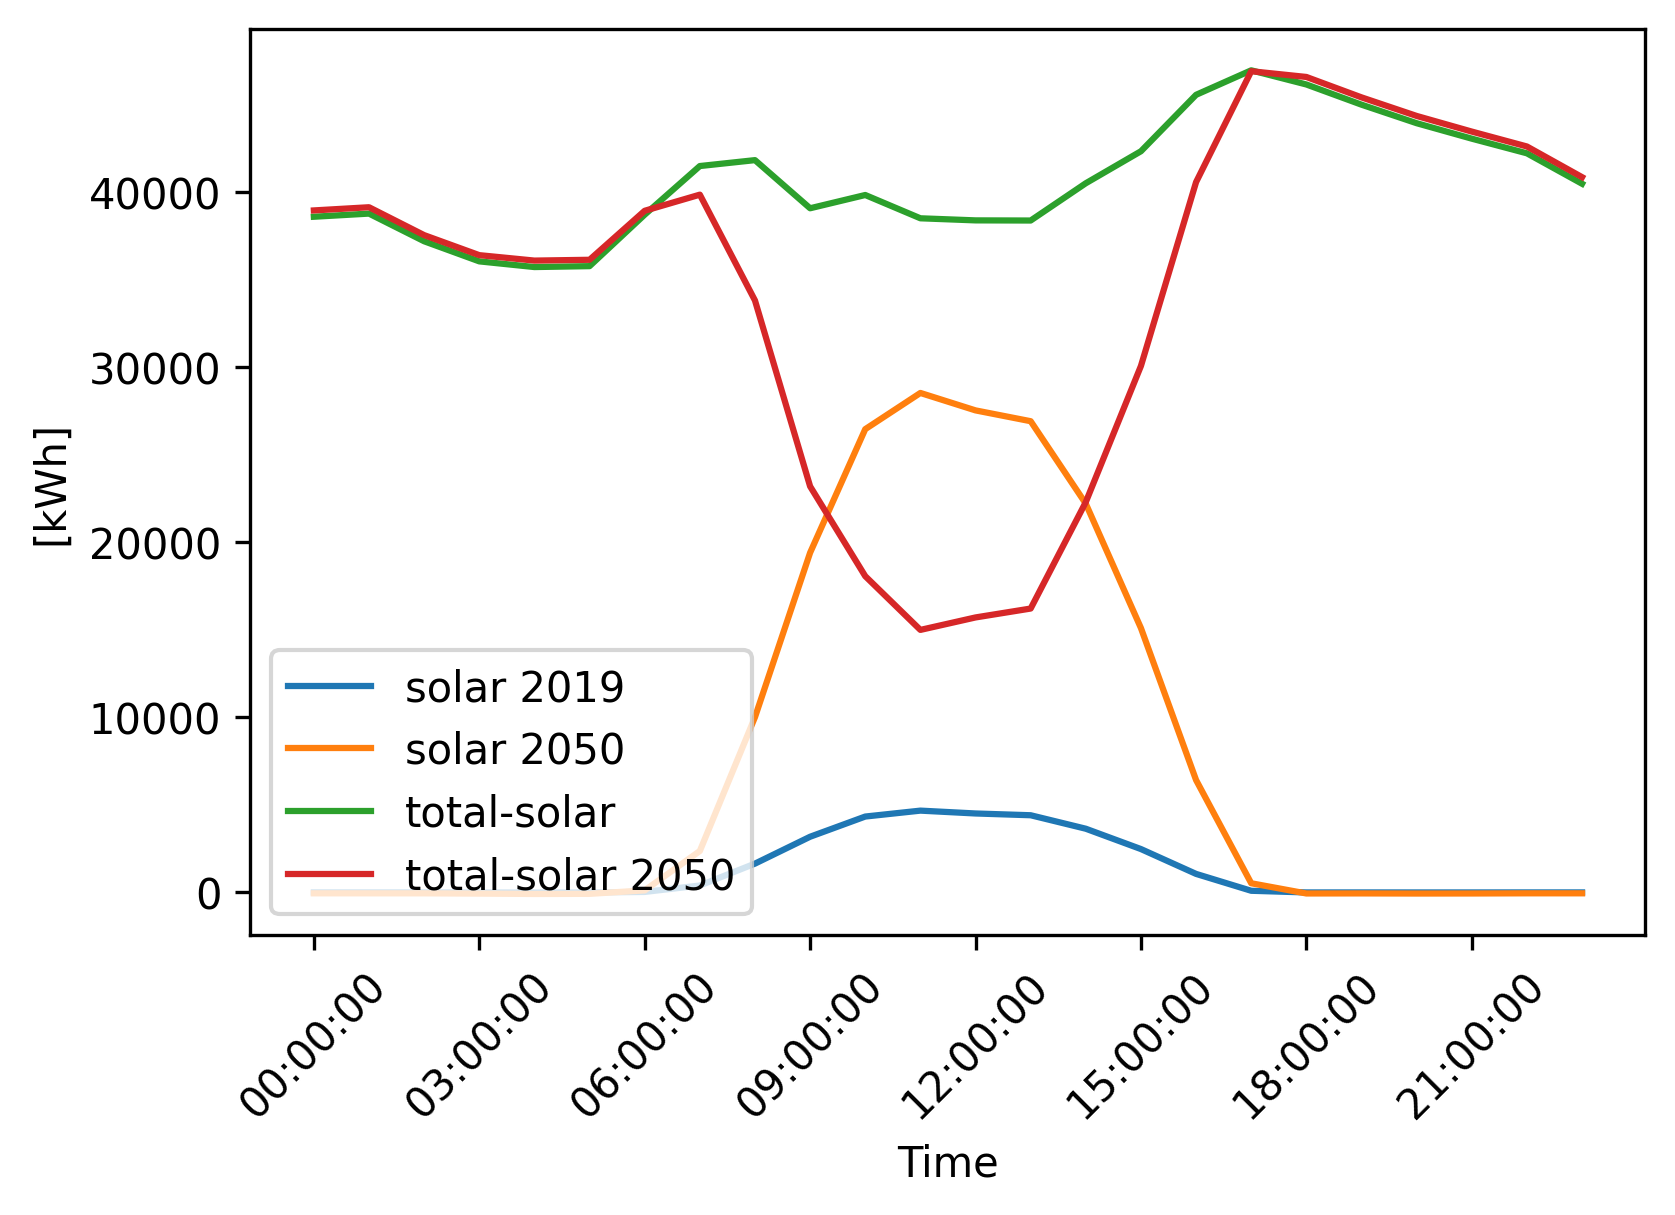
\includegraphics[height=4.0cm]{images/uiuc-duck}
		\end{center}
		\caption{Prediction on UIUC's demand for 2050.}
	\end{figure}

    \column[t]{5.5cm}
    \begin{itemize}
 		\item Spring: solar production is higher, total demand is low.
 		\item Solar generation peaked on April 4, 2019.
 		\item Peak demand is 46.9 MWh at 5 P.M.
 		\item Lowest demand is 15 MWh at 11 A.M.
 		\item Requires an installed capacity of 31.9 MW of dispatchable sources.
 	\end{itemize}

\end{columns}
\end{frame}


\begin{frame}
\frametitle{Duck curve}
\begin{columns}
    \column[t]{5.5cm}
	\begin{figure}[htbp!]
		\begin{center}
			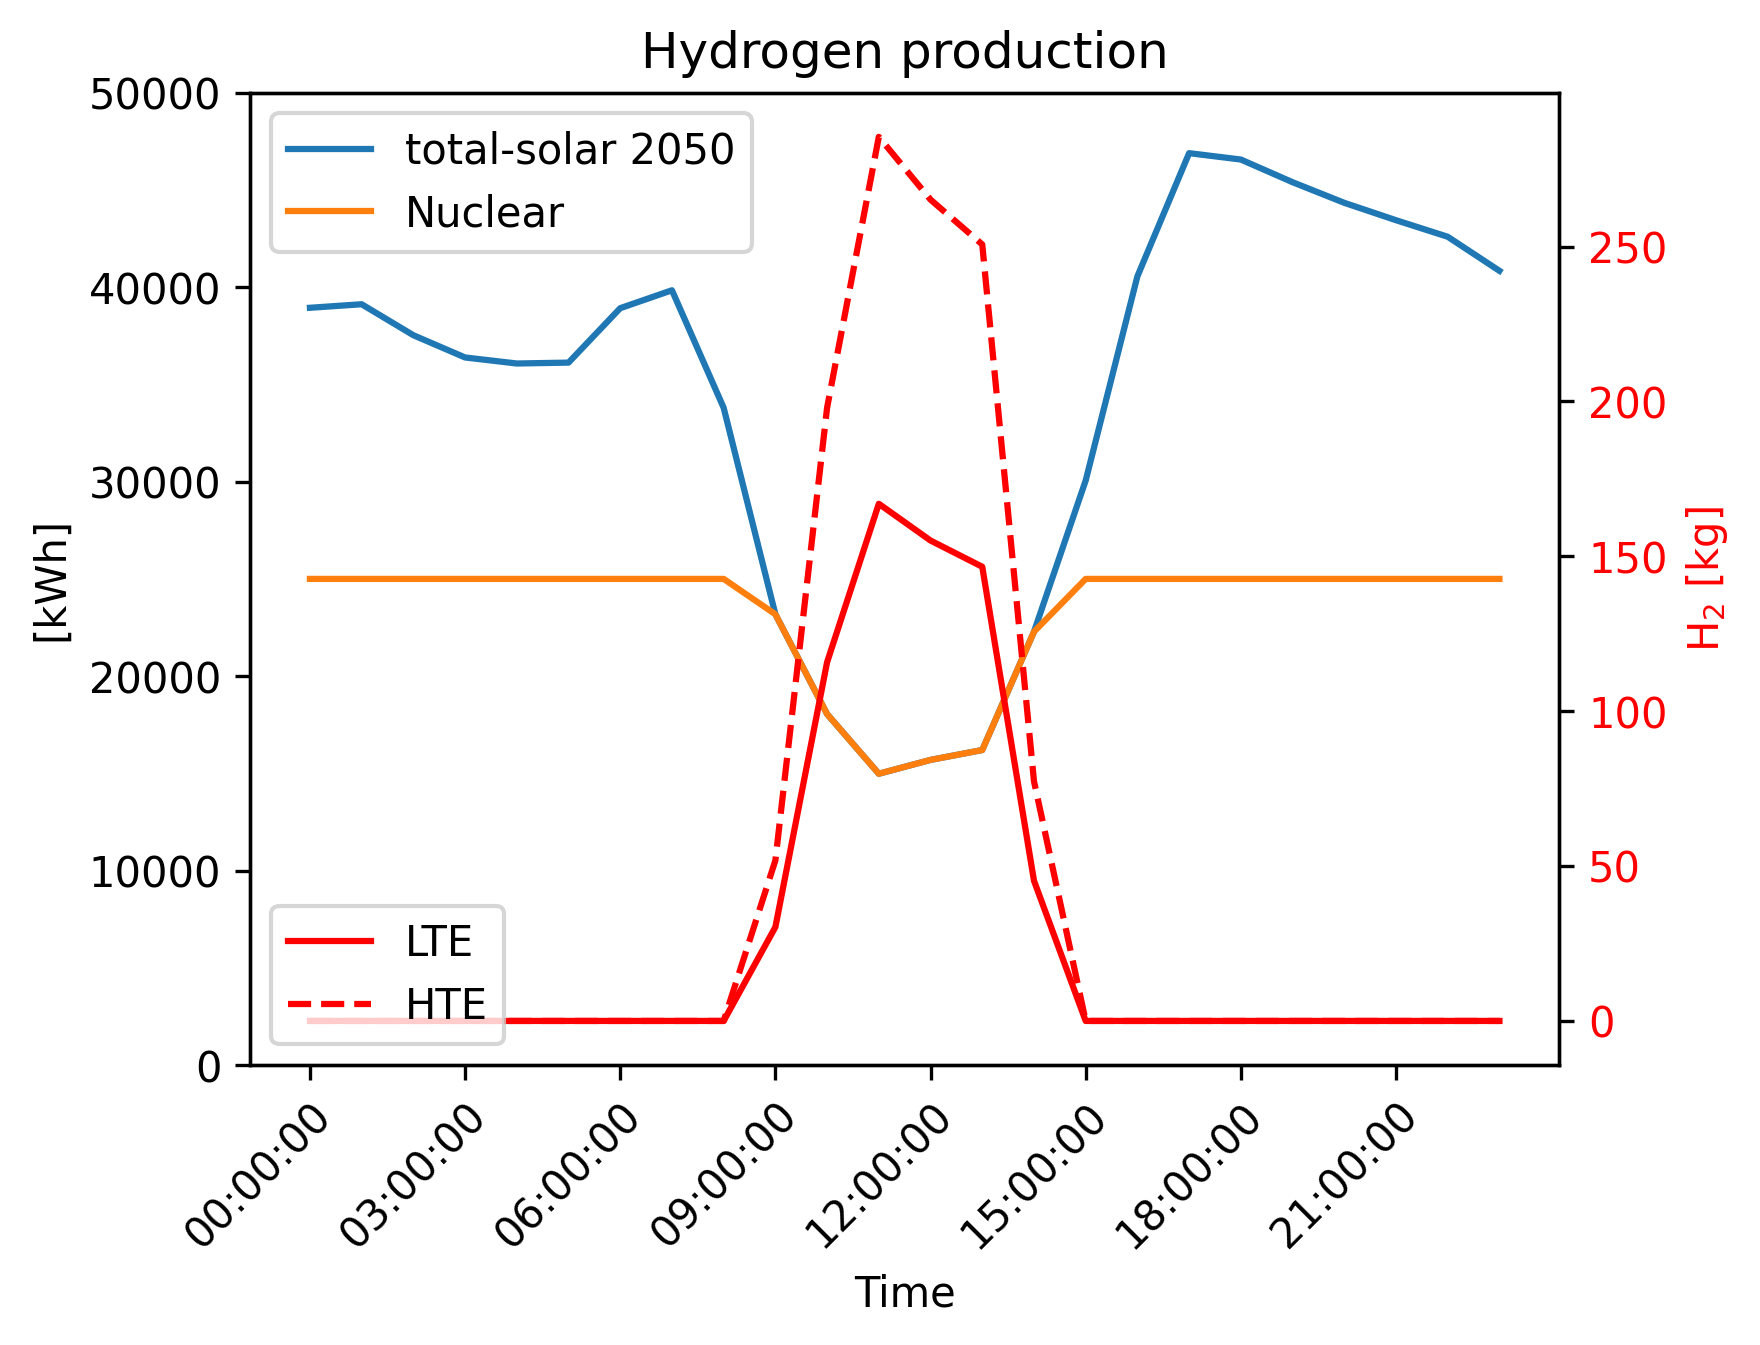
\includegraphics[height=4.4cm]{images/uiuc-hydro2}
		\end{center}
		\caption{Hydrogen production with the excess of energy.}
	\end{figure}

    \column[t]{4.5cm}
    25 MWe reactor. \vspace{0.7cm}

    LTE:
    \begin{itemize}
 		\item $\eta$=33$\%$.
 		\item 660 kg-H$_2$.
 	\end{itemize}
    \vspace{0.7cm}

    HTE:
    \begin{itemize}
 		\item HTGR.
 		\item T$_o$ = 850$^\circ$C.
 		\item $\eta$=49.8$\%$
 		\item 1136 kg-H$_2$.
 	\end{itemize}

\end{columns}
\end{frame}

\begin{frame}
\frametitle{Hydrogen for energy storage}
\begin{columns}
    \column[t]{5cm}
	\begin{figure}[htbp!]
		\begin{center}
			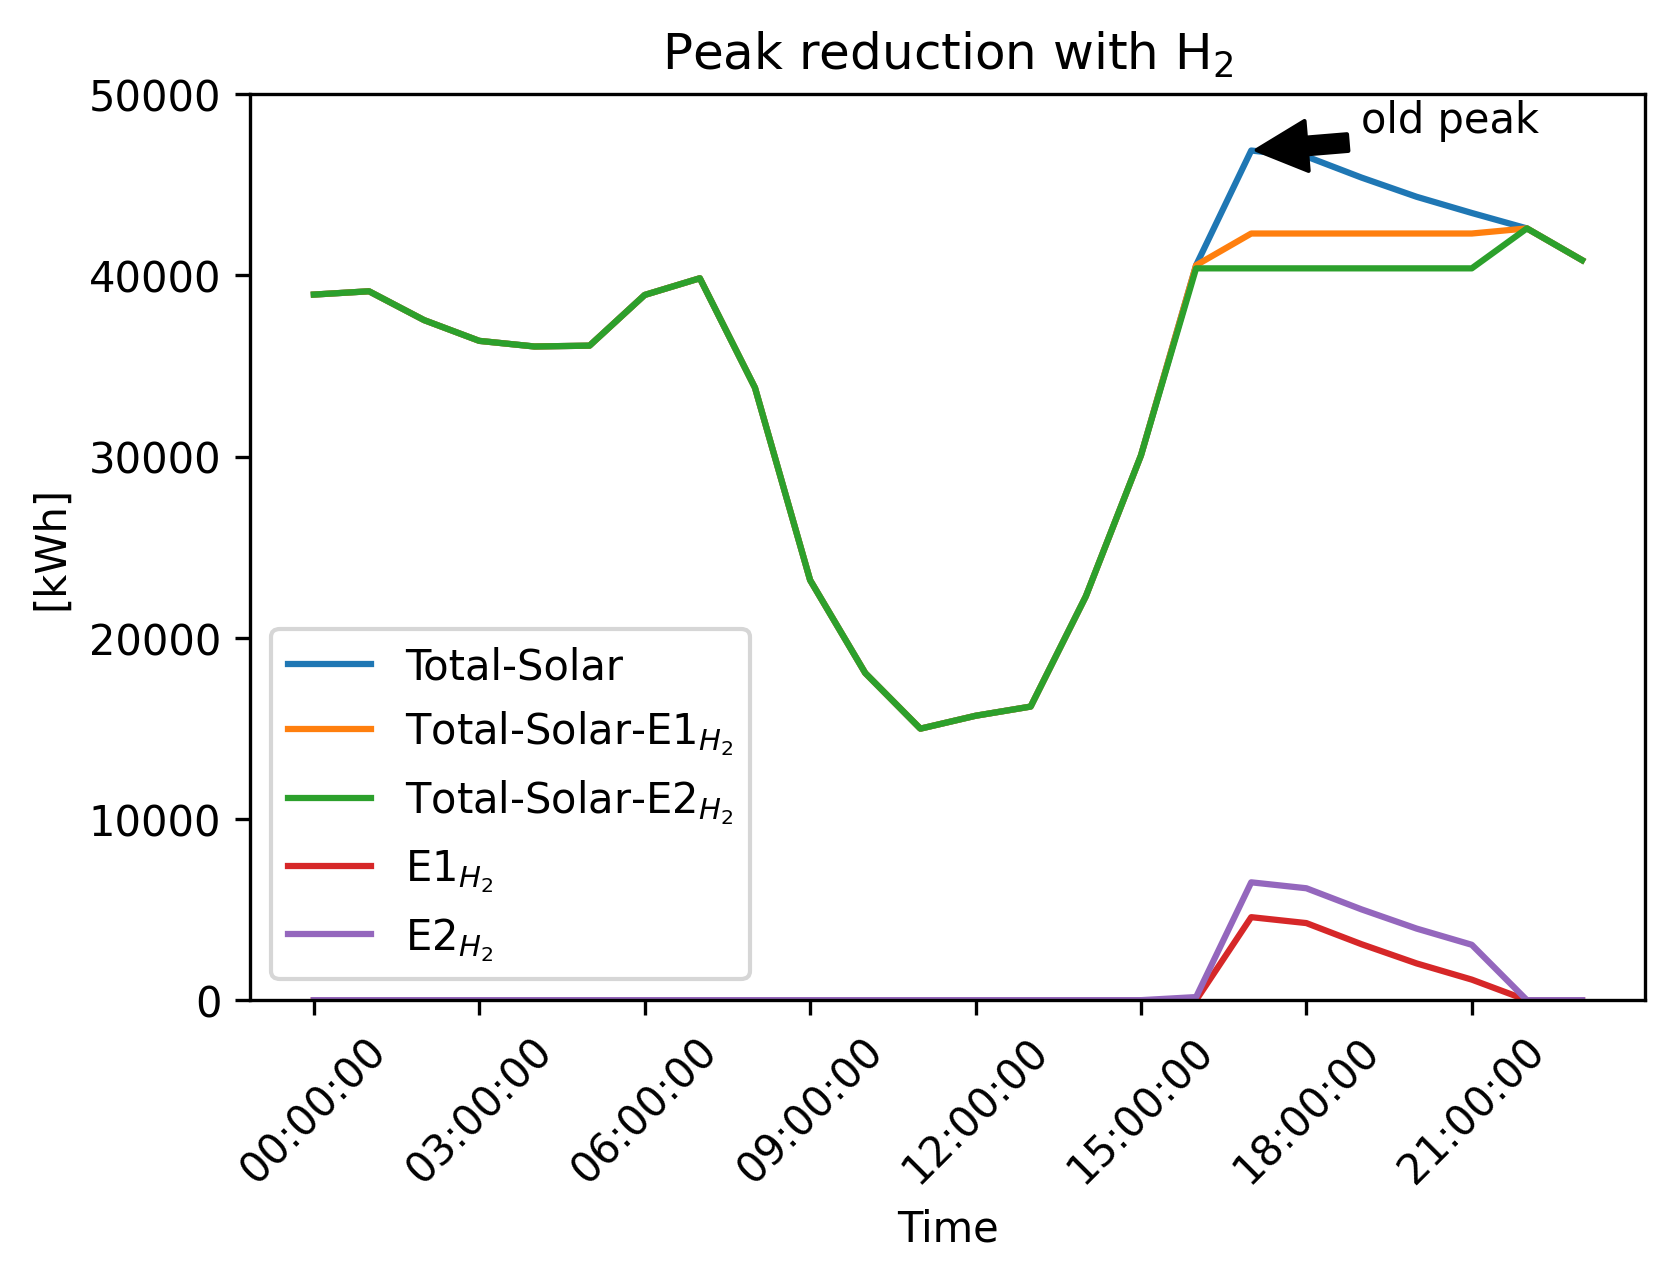
\includegraphics[height=4.4cm]{images/uiuc-hydro3}
		\end{center}
		\caption{Peak reduction by using the produced H$_2$.}
	\end{figure}

    \column[t]{4.5cm}
    \\
    LTE:
    \begin{itemize}
 		\item 15.9 MWh.
 		\item New peak: 41.9 MWh
 		\item Peak reduction: 5 MWh
 	\end{itemize}
    \vspace{0.7cm}

    HTE:
    \begin{itemize}
		\item 27.3 MWh.
		\item New peak: 40.0 MWh
        \item Peak reduction: 6.9 MWh
 	\end{itemize}

\end{columns}
\end{frame}

%%%%%%%%%%%%%%%%%%%%%%%%%%%%%%%%%%%%%%%%%%%%%%%%%%%%%%%%%%%%%%%%%%%%%%%%%%%%%%%%
\section{Conclusions}

In this work we demonstrated the \texttt{RAVEN} tool's scenario generation
capability. Ott et. al and others have shown that reservoir computing can be a
powerful method for predicting the evolution of dynamic, chaotic, systems
\cite{pathak_model-free_2018,wikner_combining_2020,bianchi_reservoir_2020}.
Accurate predictions of chaotic systems, like wind energy production, will
enable nuclear power plants to maintain their economic feasibility.
Knowledge, in advance, of renewable electricity generation will enable
operators to ramp the reactor power within the constraints given by reactor
physics. 


%%%%%%%%%%%%%%%%%%%%%%%%%%%%%%%%%%%%%%%%%%%%%%%%%%%%%%%%%%%%%%%%%%%%%%%%%%%%%%%%
\section{Acknowledgments}

This work was made possible with data provided by UIUC
Facilities and Services, in particular, Morgan White, Mike Marquissee, and Mike Larson. Additionally, this project is funded by NRC Graduate
Fellowship program.
Prof. Huff is supported by the Nuclear Regulatory Commission Faculty
Development Program (award NRC-HQ-84-14-G-0054 Program B), the Blue Waters
sustained-petascale computing project supported by the National Science
Foundation (awards OCI-0725070 and ACI-1238993) and the state of Illinois,
the DOE ARPA-E MEITNER Program (award DE-AR0000983), the DOE H2@Scale
Program (award ), and the International Institute for Carbon Neutral Energy
Research (WPI-I2CNER), sponsored by the Japanese Ministry of Education,
Culture, Sports, Science and Technology.



%%%%%%%%%%%%%%%%%%%%%%%%%%%%%%%%%%%%%%%%%%%%%%%%%%%%%%%%%%%%%%%%%%%%%%%%%%%%%%%%
\bibliographystyle{ans}
\bibliography{bibliography}
\end{document}

